% Compile with XeLaTeX:  xelatex report.tex
% Uses fontspec (Times via TeX Gyre Termes). Single-column, one-sided A4.
\documentclass[10pt,oneside,a4paper]{article}

\usepackage{fontspec}
\setmainfont{TeX Gyre Termes}[Ligatures=TeX]   % Times-compatible; swap to "Times New Roman" if installed
\setmonofont{TeX Gyre Cursor}                  % Courier-compatible monospace

\usepackage[a4paper,margin=2cm]{geometry}
\usepackage{amsmath}
\usepackage{graphicx}
\usepackage{booktabs}
\usepackage{caption}
\usepackage{enumitem}
\usepackage{titlesec}
\usepackage[hidelinks]{hyperref}

\graphicspath{{figures/}}
\captionsetup{font=small,labelfont=bf,skip=4pt}
\setlist[itemize]{noitemsep,topsep=2pt,leftmargin=1.4em}
\titlespacing*{\section}{0pt}{8pt}{3pt}
\titleformat{\section}{\normalfont\large\bfseries}{\thesection.}{0.5em}{}

\title{Multimodal RAG + Knowledge Graph over PubLayNet}
\author{Mezbaul Haque\\[2pt]\small\texttt{mezba109@gmail.com}}
\date{June 2026}

\begin{document}
\maketitle
\vspace{-1.6em}

\section{Problem formulation}

Answer scientific questions over document pages by retrieving and reasoning across
\textbf{text and visual} elements, augmenting retrieval with a small \textbf{knowledge
graph (KG)}, and producing \textbf{explainable}, cited answers. The central question
is whether non-text modality (figures/tables) and structured knowledge measurably
beat a \textbf{text-only RAG baseline}, in both retrieval and answer quality. Data:
the \texttt{lhoestq/small-publaynet-wds} subset of PubLayNet (3,812 pages; 17,366
text chunks; 2,489 figure/table regions).

\section{Data preprocessing and design choices}

A \textbf{staged, resumable pipeline} writes each stage to disk and frees the GPU
before the next, so models that cannot co-reside on a 12\,GiB card load one at a
time. Stage 1 crops every labelled region, OCRs text regions (Surya), and packs
reading-order text into $\le$1.2k-char \textbf{chunks} with provenance back to
regions. Stage 1b captions a $\sim$500-crop sample of figures/tables with a VLM
(Qwen2.5-VL-3B). Stage 2 embeds chunks (BGE-M3 dense+sparse) and crops (SigLIP2)
into an embedded Qdrant store. Stage 3 extracts entities (GLiNER, zero-shot) and
relations (LLM triples) into a NetworkX graph (67{,}796 nodes; 13{,}336 labelled
relations). The result is \textbf{three aligned views} of each page---dense+sparse
text, SigLIP image vectors, a typed entity graph---sharing region-level provenance.

\section{Architecture (baseline vs.\ enhanced)}

One retriever implements both arms; four flags select channels
(\texttt{use\_sparse / use\_image / use\_graph / use\_rerank}), so the only variables
under study are modality and structured knowledge.
\begin{itemize}
  \item \textbf{Baseline}---dense text retrieval only.
  \item \textbf{Enhanced}---dense+sparse hybrid text \textbf{+} SigLIP2
        text$\rightarrow$image figure retrieval \textbf{+} KG neighbour expansion
        \textbf{+} cross-encoder reranking.
\end{itemize}

\begin{figure}[h]
  \centering
  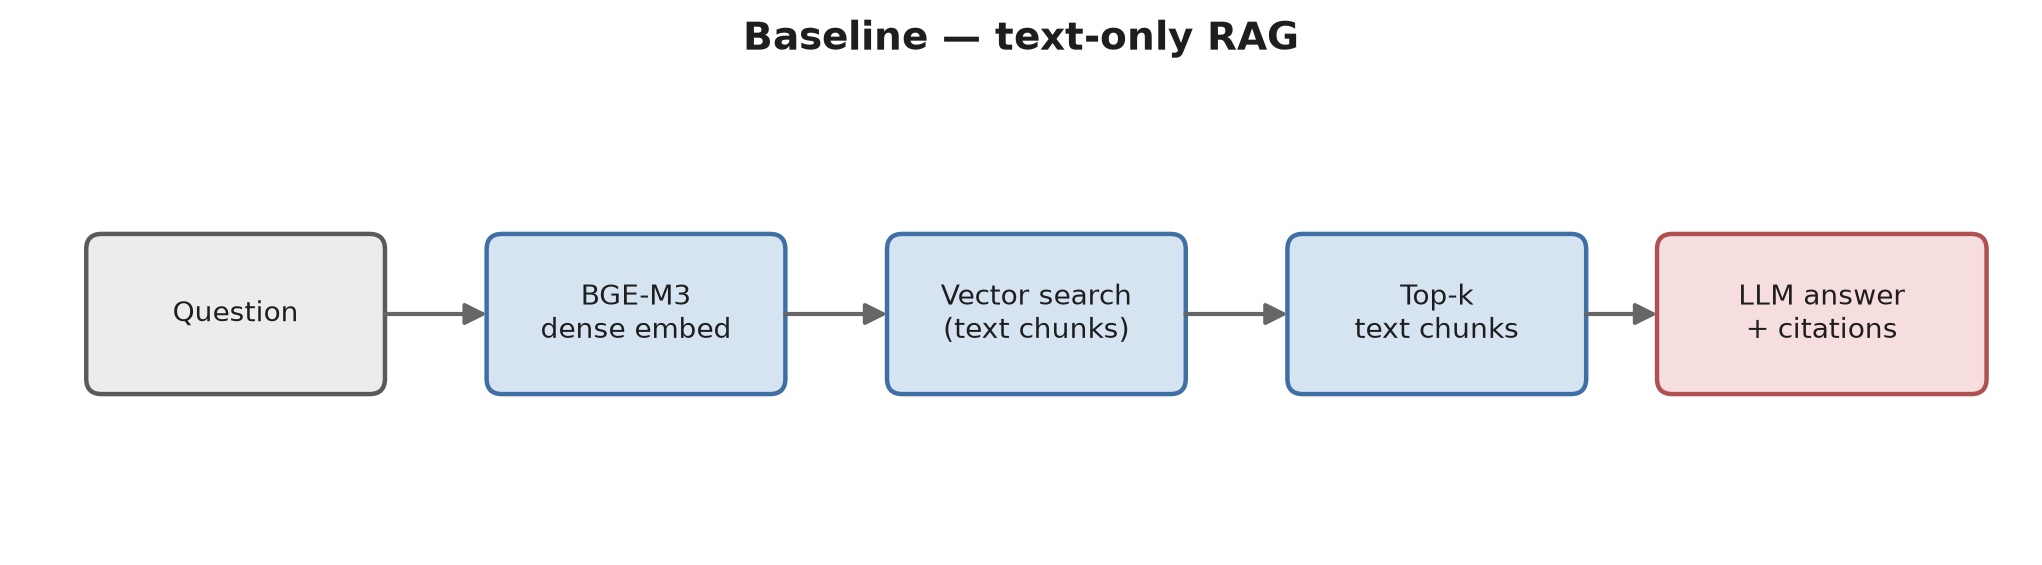
\includegraphics[width=0.78\linewidth]{architecture-baseline.png}
  \caption{Baseline: dense text retrieval feeds the generator.}
\end{figure}

\begin{figure}[h]
  \centering
  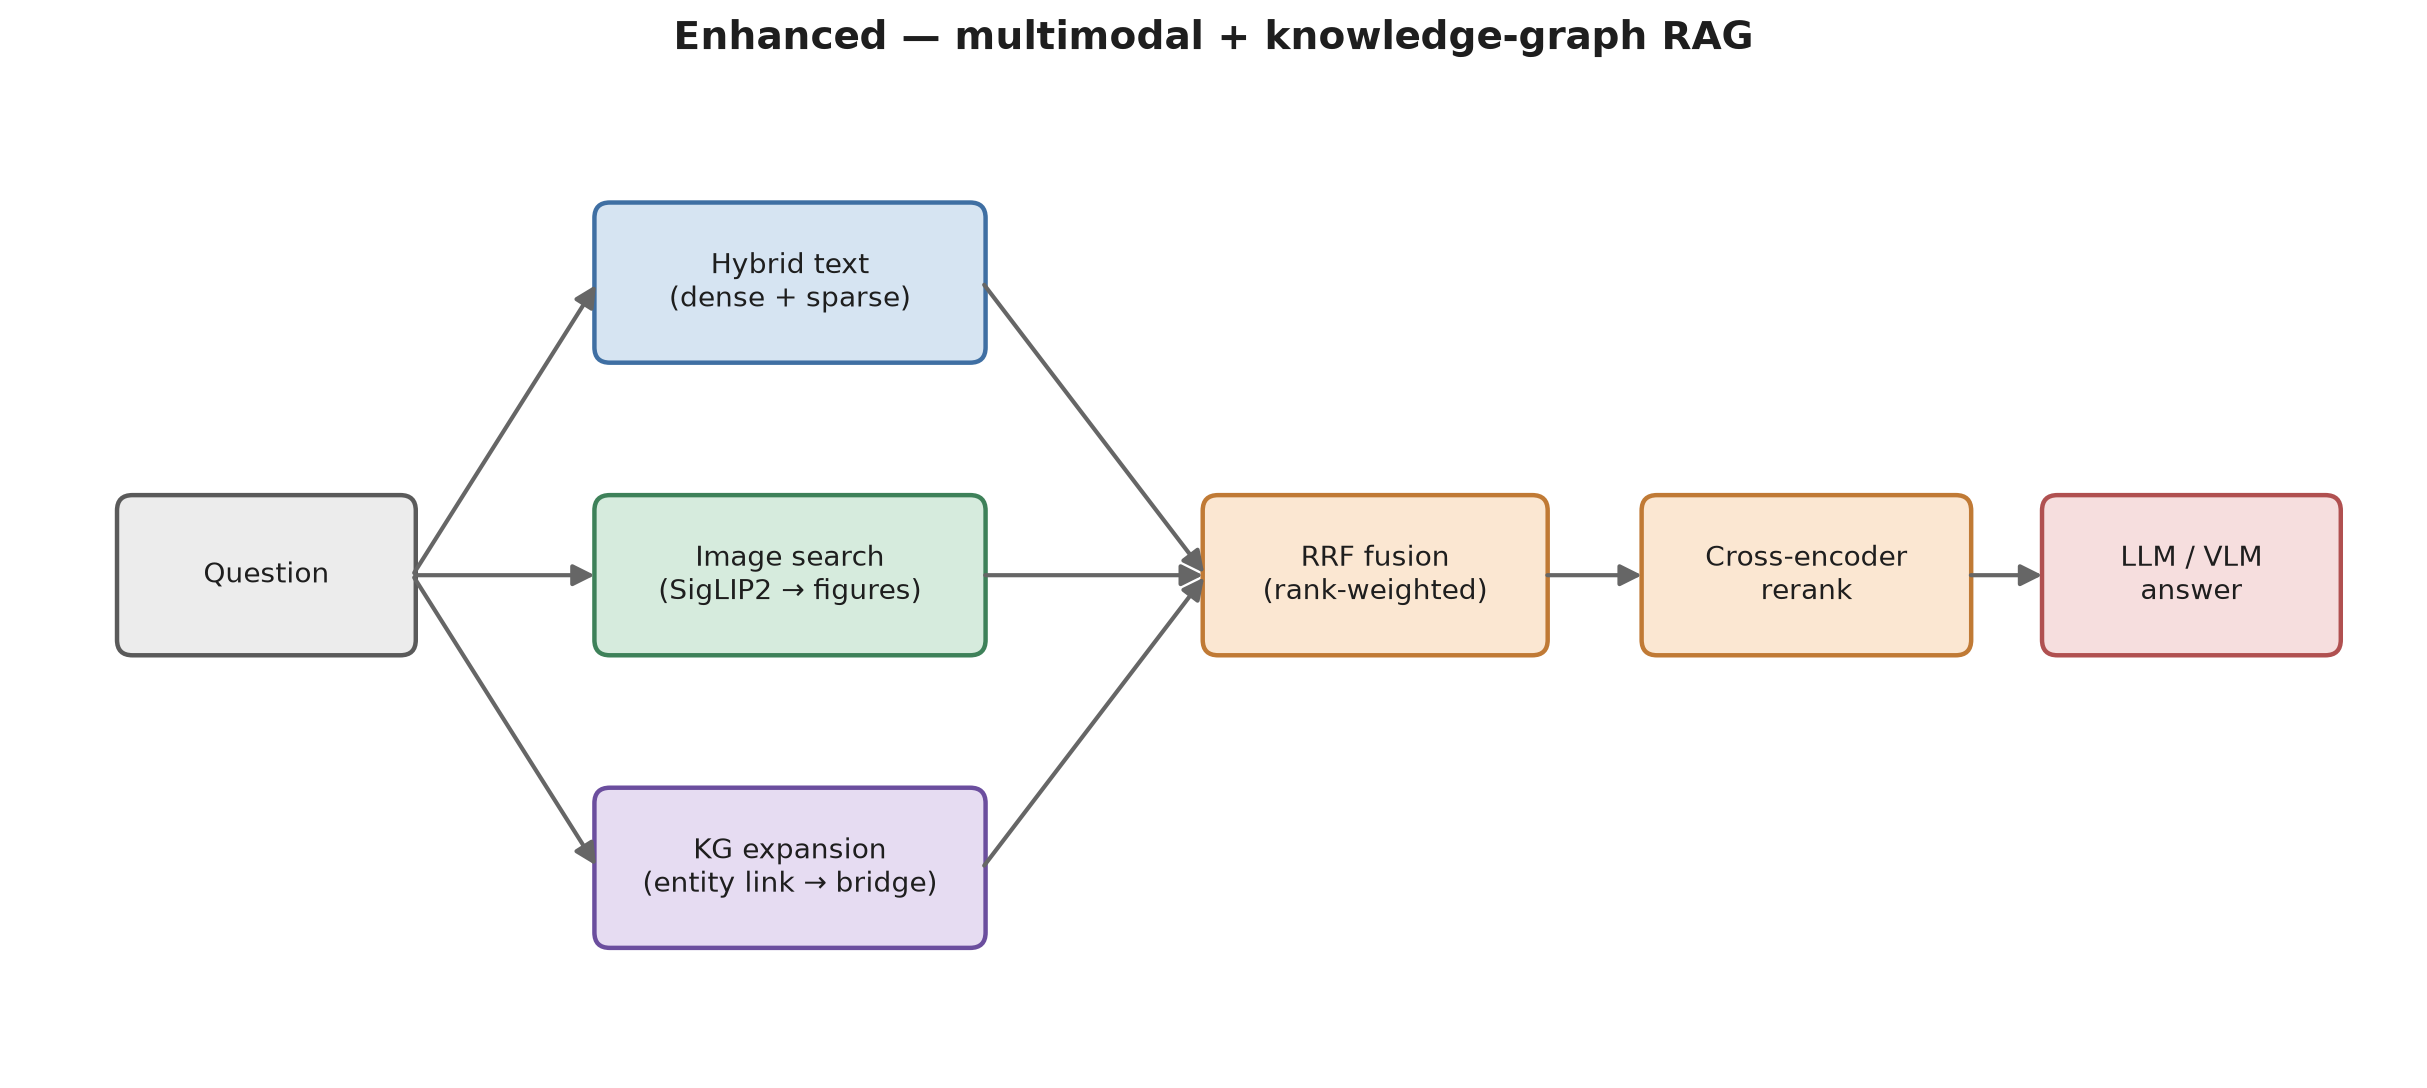
\includegraphics[width=0.95\linewidth]{architecture-enhanced.png}
  \caption{Enhanced: three retrieval channels are fused by rank-weighted RRF,
  reranked, then generated.}
\end{figure}

\textbf{Fusion by Reciprocal Rank Fusion (RRF)} is the central design choice. Each
channel returns a ranked list; fused score $=\sum w/(k+\mathrm{rank})$. Channel raw
scores are on incomparable scales (BGE cosine, SigLIP cosine, graph proximity), so
the original raw-score merge sorted every image and graph hit \emph{below} all text
hits---leaving them inert. RRF fuses by rank, so a top figure or graph-reached bridge
chunk reaches the top-$k$; the reranker then rescores the fused pool for calibrated
cross-modal order. \textbf{KG retrieval (GraphRAG-style):} a query links to its most
\emph{specific} entities (whole-word, dropping ones in $>$40 chunks as too generic),
the 1-hop neighbourhood expands, and chunks mentioning reached entities rank by
proximity---surfacing a bridge chunk vector search misses. \textbf{Reasoning /
explainability:} generation (Qwen3-4B) answers only from numbered, cited evidence;
each answer yields a provenance record (modality, channel, score, citation) plus KG
paths and cited crops. Serving/the demo can instead generate with a \textbf{VLM that
reads the crops directly} (true visual QA); the evaluation keeps the text generator
for comparable numbers.

\section{Experiments and evaluation methodology}

PubLayNet ships no QA, so we synthesise a grounded set (same LLM/corpus for both
arms). The key point is \textbf{segmented} evaluation: a single text-gold set cannot
reveal visual or graph value, so we score three typed splits, each with the gold its
channel targets:
\begin{itemize}
  \item \textbf{text} (300\,Q)---gold $=$ source chunk $\rightarrow$ text retrieval.
  \item \textbf{visual} (100\,Q)---question authored from a figure/table caption;
        gold $=$ that region $\rightarrow$ image retrieval.
  \item \textbf{multihop} (41\,Q)---names entity A but is answered by a chunk about a
        graph-neighbour B that omits A; gold $=$ that bridge chunk. \textbf{Verified}
        per question (baseline dense misses the gold \emph{and} graph expansion
        reaches it), so the split genuinely requires multi-hop retrieval.
\end{itemize}

Retrieval metrics (Recall@$k$/MRR/nDCG) run over every question, with exact-id match
on the visual/multihop splits (a same-document sibling is not a figure answer) and a
document fallback only for text. Generation metrics (faithfulness, answer-relevancy)
use an in-process LLM judge per split. We run \texttt{baseline}, four single-channel
ablations, and \texttt{enhanced}.

\section{Key results}

\begin{table}[h]
  \centering
  \caption{Retrieval (Recall@5 / MRR).}
  \begin{tabular}{lccc}
    \toprule
    Split (N) & Baseline & Enhanced & Best single channel \\
    \midrule
    text (300)              & 0.97 / 0.85 & \textbf{1.00 / 0.93} & rerank 0.98 / 0.92 \\
    visual (100)            & 0.00 / 0.00 & \textbf{0.56 / 0.54} & image 0.35 / 0.16 \\
    multihop (41)           & 0.00 / 0.00 & \textbf{0.73 / 0.54} & graph 0.61 / 0.38 \\
    \textbf{overall (441)}  & 0.66 / 0.58 & \textbf{0.87 / 0.81} & --- \\
    \bottomrule
  \end{tabular}
\end{table}

The text-only baseline scores \textbf{exactly 0} on visual and multihop---it cannot
retrieve a figure, and the multihop golds are (by construction) outside its top-$k$.
Modality and structure lift these to 0.56 and 0.73 Recall@5. \textbf{Ablations
attribute the gains cleanly:} \emph{all} visual recall is the image channel (every
text-side ablation stays 0); multihop is led by the \textbf{graph} (0.61) with sparse
(0.41) and rerank (0.46) also recovering bridge chunks; \textbf{rerank} drives the
text gain (R@1 0.75$\rightarrow$0.87). Fusion is the enabler---RRF surfaces a
figure/bridge chunk into the pool and the reranker promotes it to rank~1 (visual R@1
0.00$\rightarrow$\textbf{0.53}).

\begin{table}[h]
  \centering
  \caption{Generation (faithfulness / answer-relevancy), baseline $\rightarrow$ enhanced.}
  \begin{tabular}{lcc}
    \toprule
    Split & Baseline & Enhanced \\
    \midrule
    text     & 0.83 / 0.90 & 0.72 / \textbf{0.94} \\
    visual   & 0.45 / 0.45 & \textbf{0.49 / 0.57} \\
    multihop & 0.37 / 0.38 & \textbf{0.41 / 0.60} \\
    \bottomrule
  \end{tabular}
\end{table}

Reasoning tracks retrieval: answer-relevancy rises on every split (most on multihop,
0.38$\rightarrow$0.60) once the right evidence is retrieved. Pure-text faithfulness
dips (0.83$\rightarrow$0.72) as cross-modal context adds some off-topic
evidence---a cost of fusing modalities without routing.

\section{Discussion on the value of multimodal + KG, limitations, and insights}

\textbf{Value.} Each non-text channel unlocks a question class the baseline cannot
answer \emph{at all} (visual 0$\rightarrow$0.56; multihop 0$\rightarrow$0.73)---%
categorical, not marginal. These signals existed before but were inert under
raw-score merging; \textbf{rank-based RRF fusion} converts them into gains, so the
fusion \emph{mechanism} matters as much as the channels.

\textbf{Insights.} (1)~A text-gold-only benchmark structurally hides multimodal/KG
value---segmented evaluation is essential. (2)~Graph and sparse retrieval are partly
redundant on multi-hop, but the graph captures most (0.61 vs 0.41) by reaching chunks
sharing \emph{no} surface terms with the query. (3)~Equal-weight fusion trades a
little text precision for large cross-modal recall (overall R@1
0.51$\rightarrow$0.76); a per-query router is the clear next step.

\textbf{Limitations.} Small subset; $\sim$500 captioned crops; a simple self-judge
(not RAGAS); the multihop split is synthetic and verified by construction (it
measures \emph{recoverability} of graph-required evidence); SigLIP/captioner are
general-purpose; no query routing or fine-tuning (out of scope). On \emph{answer}
quality, retrieval cites the correct figure but exact table reading is bounded by
\textbf{table-VQA, not the pipeline}: on a dense HER2/EC50 table (PMC5384386, p.2)
our 3B VLM reads HER2 max 4{,}900 correctly but misreads the EC50 max (64.9 vs the
true $>$5{,}000)---and prompted on the same table GPT and Claude also miss cells
(true HER2 min 3 vs their 4/6). Salient values are reliable; pinpoint extremes are
not, even for frontier models---the known failure mode of table understanding. The
robust fix for tables is structure OCR (parse cells $\rightarrow$ compute), not a
bigger VLM; for charts, where OCR does not apply, a sharper/stronger VLM is the lever.

\begin{figure}[h]
  \centering
  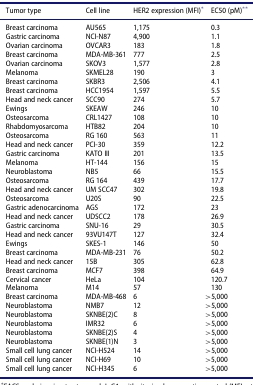
\includegraphics[width=0.22\textwidth]{her2-table.png}
  \caption{The HER2/EC50 table (PMC5384386, p.2): dense, low-resolution cells that
  even GPT and Claude misread.}
\end{figure}

\section{Reproduction}

\texttt{pip install -e .}, then run stages \texttt{01}, \texttt{01b}, \texttt{02},
\texttt{03} in order, and
\texttt{04\_run\_eval.py --variants baseline,abl\_rerank,abl\_hybrid,abl\_image,abl\_graph,enhanced}
(full commands in the README). Stages are resumable; \texttt{dev/test.sh} covers the
new logic (fusion, KG, multi-hop filter, metric segmentation) with no GPU.

\end{document}
